\subsection{Detalls d'implementació}

    \paragraph{}
    Abans de comentar en detall alguns aspectes de la implementació, volem indicar que només el fitxer del controlador, d'aquesta funcionalitat, està compost per quasi mil línies de codi i que evidentment, resulta impossible exposar totes les tasques que aquest realitza en aquesta secció.

    És per aquest motiu, que només es destaquen les interaccions principals o més importants, de cara a la interacció amb l'API i configuració de la pàgina.

    El controlador que s'encarrega de gestionar totes les interaccions de l'usuari amb la funcionalitat, es troba en el fitxer \emph{search.js}.

    \subsubsection{Iniciant la cerca de persones}

\paragraph{}
Quan l'usuari prem el botó de cerca, la primera tasca del controlador és validar que els continguts introduïts en el formulari siguin correctes. En cas que el formulari no compleixi les condicions de cerca, es dispararà un conjunt d'errors informant l'usuari de la informació a corregir i no es llençarà cap crida contra l'API.

Per realitzar aquesta validació, el formulari escapa cada camp que pot ser introduït per l'usuari i comprova si s'ha de realitzar alguna verificació específica del contingut.

Escapar el camp d'un formulari significa codificar certs caràcters especials, com per exemple, `\&', `<', `>', `/', etcètera, per tal d'assegurar el seu correcte transport pels URL i evitar atacs malintencionats, que pretenguin trencar el HTML i afectar el servidor, mitjançant injeccions de codi. El fitxer, \emph{formValidation.js}, s'encarrega de realitzar aquestes transformacions i validacions.

Mostrem a continuació, el codi que escapa els caràcters no desitjats. Per escapar un paràmetre, només cal enviar-lo contra la funció \emph{escapeHtml()}.

\begin{lstlisting}[style=rawOwn,caption={Funcio \emph{escapeHtml()} i la variable \emph{entityMap}}]
var entityMap={`&':`&amp;', `<':`&lt;', ... `/': `&#x2F;'};

function escapeHtml(string) {
    return String(string).replace(/[&<>"'\/]/g, function (s) {
        return entityMap[s];
});
}
\end{lstlisting}

Si no es mostra cap error de validació, significa que el formulari és correcte i compleix amb les condicions de cerca.

Arribats a aquest punt, es prepara l'objecte \emph{params}, que emmagatzema tots els paràmetres de cerca descrits a l'últim apartat de la secció cinc de la memòria, s'eliminen de la crida aquells que no han estat introduïts per l'usuari i es demana la cerca dels primers quinze resultats mitjançant la crida a la funció \emph{print\-Persons\-To\-Table(0)}.

    \subsubsection{La funció printPersonsToTable()}

\paragraph{}
Aquesta funció, acaba de configurar els paràmetres necessaris per poder realitzar la cerca, la llença i en tracte la resposta.

En concret, configura els paràmetres \emph{inici} i \emph{context} i tot seguit, llença la crida asíncrona cap al SDK. Aquests paràmetres, ja han estat descrits en seccions anteriors de la memòria, però recordem, que s'encarreguen de delimitar el primer resultat a retornar i a quina cerca es fa referència, en cas que s'estiguin demanant més blocs de resultats, d'una cerca ja realitzada contra l'API de FamilySearch.

Si no es produeix cap error, l'API retornarà els primers quinze resultats i aquests es pintaran sobre una taula. En cas contrari, l'aplicació ensenyarà l'error a l'usuari, tot indicant-ne el motiu de fallida.

\begin{lstlisting}[style=rawOwn,caption={Llençament de peticions contra el SDK i captura d'errors}]
client.getPersonSearch(params).then(function(searchResponse) {
    // Get persons and display id, name, birth date, death date
    ...
})
.catch(function(e) {
    // Display error
    ...
});
\end{lstlisting}

L'estructura de codi anterior, encarregada de llençar una petició al SDK i capturar els possibles errors, és l'estàndard que segueixen totes les crides realitzades des de la nostra aplicació web, cap al el SDK de FamilySearch.

La llista de resultats pintada en la nostra aplicació web, es mostra a la figura~\ref{fig:searchTableResults}.

\begin{figure}[h]
    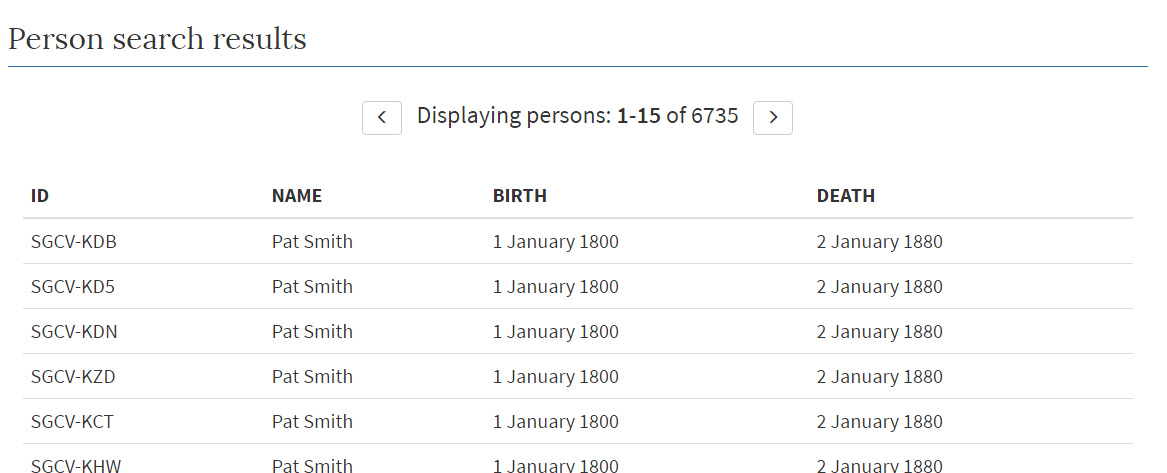
\includegraphics[width=\linewidth]{11/02_searchPersons/01_resultsTable}
    \centering
    \caption{Exemple de resultats d'una cerca a l'arbre familiar}\label{fig:searchTableResults}
\end{figure}

La gràcia de la funció \emph{printPersonsToTable(pos)} és que pot ser reutilitzada quan l'usuari vol navegar pels diferents blocs o pàgines de resultats, sense la necessitat de revalidar el formulari de cerca.

Quan el SDK retorna els resultats al controlador, aquest emmagatzema, en varia\-bles globals, els paràmetres resultats totals, índex del primer resultat mostrat i context de la cerca.

Gràcies a aquestes variables, la funció es pot encarregar de configurar els paràmetres: posició d'inici i context, just abans de realitzar la cerca contra el SDK i per tant, ser reutilitzada amb facilitat, conjuntament a l'objecte \emph{params}, per demanar més blocs de resultats d'una cerca ja realitzada.

\begin{lstlisting}[style=rawOwn,caption={Actualització i utilització dels parametres \emph{count}, \emph{start} i \emph{context}}]
function printPersonsToTable(pos) {
    // Update start params
    params.start = pos;
    params.context = context;

    // Search with the defined parameters
    client.getPersonSearch(params).then(function(searchResponse) {
        // Get parameters
        count = searchResponse.getResultsCount();
        start = searchResponse.getIndex();
        context = searchResponse.getContext();
        ... // tractament dels resultats
    });
}
\end{lstlisting}

    \subsubsection{Mostrant els detalls d'una persona}

\paragraph{}
La selecció d'una persona des de la taula de resultats originada per la cerca, provoca una segona crida al SDK de FamilySearch, en la que s'obté tota la informació disponible sobre la persona seleccionada i els seus familiars més propers.

Com en totes les crides a l'API, en cas d'error, aquest és mostrat en una secció específica de la interfície d'usuari.

En cas d'èxit, es pinta, en diferents taules, la informació bàsica de la persona, els diferents noms pels quals és coneguda, els esdeveniments relacionats amb la seva vida, informació bàsica sobre els seus pares, parelles i fills, informació de la seva ascendència i descendència, notes de FamilySearch, fonts de dades que verifiquen la informació mostrada i l'historial de canvis realitzat sobre la persona.

Es mostra en la figura~\ref{fig:personSearchDetails}, l'inici de la secció de taules, resultant de demanar els detalls específics d'una persona.

\begin{figure}[h]
    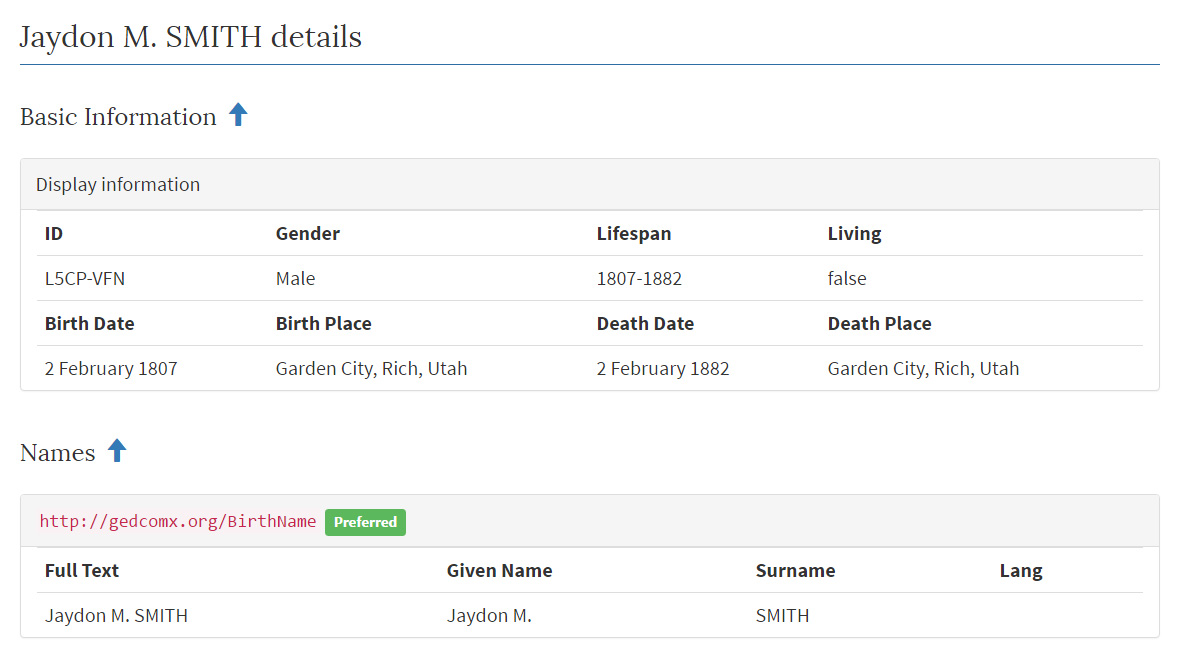
\includegraphics[width=\linewidth]{11/02_searchPersons/02_personDetails}
    \centering
    \caption{Exemples de l'inici dels detalls d'una persona}\label{fig:personSearchDetails}
\end{figure}

La crida a l'API que gestiona aquesta informació és mostra en el següent bloc de codi.

\begin{lstlisting}[style=rawOwn,caption={Crida al SDK per obtenir tota la informació d'una persona}]
client.getPersonWithRelationships(personID).then(function(personResponse) {
    var mainPerson = personResponse.getPrimaryPerson();
    personDisplayProperties(mainPerson);
    personDisplayNames(mainPerson.getNames());
    personDisplayFacts(mainPerson.getFacts());
    ...
    client.getAncestry( ... );
    client.getDescendancy( ... );
    ...
    mainPerson.getChanges( ... );
});
\end{lstlisting}

Com s'ha pogut observar en el bloc de codi anterior, per obtenir les diferents peces d'informació, s'ha de navegar per diferents nivells de la resposta. Alguna informació és accessible directament des de l'objecte inicial, mentre que alguns paràmetres, cal anar a buscar-los a l'objecte específic de la persona. Per altra banda, la informació relativa a l'ascendència i descendència, cal demanar-la de forma explícita al SDK, amb un parell de crides extra.

Les dades retornades sobre l'ascendència i descendència, esdevenen interessants, ja que la navegació pels resultats es realitza de forma diferent. En concret, mitjançant les nomenclatures `Ahnentafel' i `Aboville', respectivament.

La nomenclatura `Anhentafel', atorga a la persona sobre la qual se cerca l'as\-cen\-dèn\-cia, el nombre 1. El seu pare, rep el número 2 i la mare, el 3. Les regles per calcular els nombres dels pares, de qualsevol persona en l'ascendència, són:

\begin{itemize}
    \item \textbf{Pare:} nombre de la persona $\times$ 2
    \item \textbf{Mare:} nombre de la persona $\times$ 2 + 1
\end{itemize}

Per altra banda, la nomenclatura `Aboville', utilitza una estructura similar a la de les seccions i apartats d'aquesta memòria. Si s'atorga el nombre 1, a la persona sobre la qual se cerca la descendència, s'utilitza per les diferents generacions:

\begin{itemize}
    \item \textbf{Fills:} 1.1 / 1.2 / 1.3 / etcètera.
    \item \textbf{Els fills dels fill 1.1:} 1.1.1 / 1.1.2 / 1.1.3 / etcètera.
    \item \textbf{Els fills del fill 1.2 del fill 1.1:} 1.1.2.1 / 1.1.2.2 / etcètera.
\end{itemize}

    \subsubsection{Generació de taules dinàmiques amb informació sobre un recurs}

\paragraph{}
Com s'ha especificat en l'apartat anterior, la informació referent als diversos recursos disponibles dels detalls d'una persona, s'imprimeix en diferents taules.

La idea de com representar aquestes taules neix de l'aplicació d'exemple del SDK de Javascript\footfullcite{createPanel}. Mitjançant l'adaptació del codi d'aquest, ajustant-lo a les necessitats del nostre projecte, s'aconsegueix, mitjançant la combinació de Bootstrap, javascript i jQuery, la generació de taules dinàmiques.

Es requereixen taules dinàmiques, ja que el nombre d'entrades en recursos com l'historial de canvis o el nombre de fills d'una parella, no és estàndard i per tant, s'ha d'adaptar per cada persona en concret.

La generació de les taules es realitza mitjançant la creació de matrius de dades, on cada cel·la és composta per un vector de dos valors. El primer, indica el tipus del camp de la cel·la, mentre que el segon, el contingut.

Mostrem en el següent bloc de codi, les dues primeres fileres de la matriu de dades relativa a la informació bàsica d'una persona.

\begin{lstlisting}[style=rawOwn,caption={Exemple de les dues primeres files, d'una matriu de dades}]
var displayProperties = createPanelTable(`Display information', [
    [
        [`th', `ID'],
        [`th', `Gender'],
        [`th', `Lifespan'],
        [`th', `Living']
    ],
    [
        [`td', person.getId()],
        [`td', person.getDisplayGender()],
        [`td', person.getDisplayLifeSpan()],
        [`td', person.isLiving()]
    ], ...
];
\end{lstlisting}

Un cop s'han creat les diferents matrius de dades, s'utilitza la funció \emph{create\-Panel\-Table(header, rows)}, per transformar-les en un bloc de codi HTML, que pinti les taules dins d'un panell de Bootstrap. Tot seguit, mostrem el codi que tradueix el bloc principal de files a HTML.

\begin{lstlisting}[style=rawOwn,caption={Transformació de files d'una matriu en HTML}]
for(var i = 0; i < rows.length; i++){
    var $row = $(`<tr>').appendTo($table);
    for(var j = 0; j < rows[i].length; j++){
        $(`<'+rows[i][j][0]+`>').text(rows[i][j][1]).appendTo($row);
    }
}
\end{lstlisting}

